\begin{minipage}[t]{180mm}
\fcolorbox{black}{white}{
\begin{minipage}[b]{30mm}

\includegraphics[width=0.5\linewidth]{unflogo.pdf}
\end{minipage}
\begin{minipage}[b]{100mm}
\Huge \textbf{UNF NEWZ} \\
\Large -- Stadig uden nok søvn!
\end{minipage}
\begin{minipage}[b]{50mm}
\Large Fredag 19.07.2016 \\
\normalsize Redigeret i \LaTeX\ af \\ SOM, MGS
\end{minipage}
}
\end{minipage}



\begin{minipage}[b]{0.95\linewidth}
\begin{minipage}[t]{0.47\textwidth}
\vspace{1mm}
\section*{Trafikmeldinger fra Bane Danmark og DSB}
\begin{itemize}
\item På grund af sporarbejde kører der færre tog til ændrede tider over Lillebælt
\item Der kører busser mellem Roskilde Vest og Holbæk
\item Regionaltogene mellem København og Ringsted kører kun én gang i timen
\item S-tog linje E kører ikke
\item S-tog linje A mellem Vallenbsbæk og Åmarken erstattes af bus
\end{itemize}

\section*{Dagens koordinator}
Hvis du møder en koordinator, så prik ham, han vil dog ikke reagere, fordi han er for træt.

\vspace{1mm}
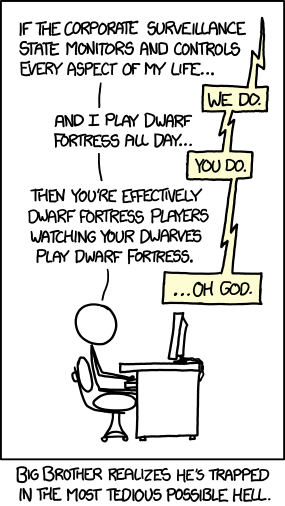
\includegraphics[width=\linewidth]{dwarf_fortress.png}
\tiny Randall Munroe, http://xkcd.com/1223/, CC-BY-SA-2.5

\end{minipage}%
\hfill\begin{minipage}[t]{0.47\textwidth}
\vspace{2mm}
\section*{Vejrudsigt}
\textbf{IMF, AU (fra DMI)}: Temperaturer fra 11 til 26 grader og høj solskin med svag vind fra skiftende retninger der minder om vest. Der forventes et moderat antal græspollen, og et lavt antal bynkepollen.

\textbf{Skagen}: Temperaturer fra 12 til 19 grader og høj sol med svag vind fra syd.

\textbf{København}: Temperaturer fra 10 til 24 grader og høj sol med vind fra nord.

\textbf{Tønder}: Temperaturer fra 11 til 23 grader og høj sol med svag vind fra nordvest.

\textbf{Bornholm}: Termperaturer fra 11 til 19 grader og høj sol med svag vind fra nordvest.

\textbf{Torshavn}: Temperaturer fra 10 til 15 grader og skyet med svag vind fra vest.

\textbf{Nuuk}: Temperaturwer fra 3 til 9 grader, skyet med lidt sol og svag vind fra nordøst.

\section*{Fakta om Jylland}
I Jylland er der lige så mange personer, der kan køre traktor, som der er personer, der er fyldt syv år

\vspace{1mm}
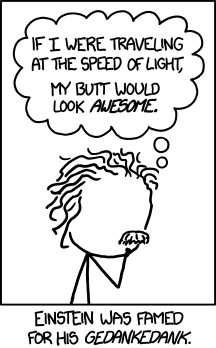
\includegraphics[width=\linewidth]{relativity.png}
\tiny Randall Munroe, http://xkcd.com/1233/, CC-BY-SA-2.5

\end{minipage}

\begin{center}
\tiny UNF Newz er avisen hvor at ansvarshavende redaktør fralægger sig ethvert ansvar for eventuel plagiering, kaniner, tysk, stavefelj, kaffe, dårlig humor, glemsomhed, katte, store sigmaer, pile, skyer, dårlige oversættelser og alt hvad eventuelle homo sapiens sapiens kunne finde på at holde imod UNF Newz! Dog tager UNF Newz fuld credit og copyright for alle guldkorn, magickort, mus, \TeX, humor, smil, Mortener, kaffe, før-fremtid, ringe og/eller Rubiksterning.
\end{center}
\end{minipage}

